\documentclass[Orbiter Developer Manual.tex]{subfiles} 
\begin{document}

\section{Spacecraft design}
This section describes how to create a new \textit{vessel class} for Orbiter by writing a \textit{vessel DLL module}. Although it is possible to create simple vessel classes by writing a vessel configuration file without a custom module, the full potential of Orbiter’s custom spacecraft design capabilities can only be realised with a specialised module.\\

\alertbox{All vessels of a given class share the same DLL module. Orbiter only loads a single instance of the DLL. This means that global variables are shared between all vessels of that class. Do not store data which are specific to individual vessels in global or static variables, because they can be overwritten by another vessel.}


\subsection{Module initialisation}
When the user launches the simulation by picking a scenario from the Orbiter Launchpad dialog and pressing the “Launch Orbiter” button, Orbiter will load the vessel DLL module for each spacecraft type used in the simulation, and call its \textit{InitModule} function. This function is called only once per Orbiter session, no matter how many spacecraft of that type appear in the simulation. It will not be called again if the user exits the simulation to the Launchpad, and reloads another simulation scenario. You can use it to initialise global (non-instance specific and non-session specific) parameters.

\begin{lstlisting}
#define ORBITER_MODULE
#include "orbitersdk.h"

HINSTANCE g_hDLL;

DLLCLBK void InitModule( HINSTANCE hModule )
{
	g_hDLL = hModule;
	// perform global module initialisation here
}
\end{lstlisting}

\noindent
In this example, we use the \textit{InitModule} function to save the module instance handle passed to the function in global variable \textit{g\_hDLL}. This handle is useful later, e.g. when loading resources stored in the module file. Note the first line of the code example, which defines the \textit{ORBITER\_MODULE} flag. This flag should be included in all Orbiter DLL modules, to ensure proper execution of initialisation and cleanup functions.\\
\\
At the end of a simulation run, Orbiter calls the \textit{ExitModule} function for each DLL module.

\begin{lstlisting}
DLLCLBK void ExitModule( HINSTANCE hModule )
{
	// perform module cleanup here
}
\end{lstlisting}

\noindent
If you performed any dynamic memory allocation in \textit{InitModule}, this is a good place to perform the corresponding cleanup operations which de-allocate that memory.


\subsection{Vessel initialisation}
To allow initialisation of individual spacecraft, Orbiter will call the ovcInit function each time a scenario is loaded, for each vessel of that type listed in the scenario file. Orbiter will also call \textit{ovcInit} during the simulation if a new vessel of this type is created. The main purpose of ovcInit is to create an instance of a \textit{VESSEL}-derived interface class. \textit{VESSEL} is a class defined in the Orbiter API which is the primary means of communication between Orbiter and your own spacecraft class. In order to make use of the interface, you should derive your own vessel class derived from \textit{VESSEL}. In \textit{ovcInit}, you then create an instance of that class and return it back to Orbiter. Note that in the latest Orbiter version, the new \textit{VESSEL2} class has been introduced which inherits all the methods of \textit{VESSEL}, and introduces a number of new callback functions which replace the previous method of event notification. You should derive your vessel class from \textit{VESSEL2} to make use of this latest interface.\\
\\
As an example, let’s create a new class called \textit{MyVessel}, and create an instance in \textit{ovcInit}:

\begin{lstlisting}
class MyVessel: public VESSEL2
{
	public:
		MyVessel( OBJHANDLE hObj, int fmodel ) : VESSEL2( hObj, fmodel ) {}
		~MyVessel() {}
		// add more vessel methods here
};

DLLCLBK VESSEL* ovcInit( OBJHANDLE hvessel, int flightmodel )
{
	return new MyVessel( hvessel, flightmodel );
}
\end{lstlisting}

\noindent
\textit{ovcInit} passes two parameters to your module: a handle to the vessel for which you are about to create an interface, and a flag for the type of flight model requested by the user. Both parameters are passed on to the vessel constructor. The vessel handle is required to identify your vessel when requesting information from Orbiter. The \textit{flightmodel} flag can be used to implement different behaviour in your module, for example to define an “easy” and a “complex” flight model, which can then be selected by the user. You don’t need to store these parameters in your module, because you can retrieve them with the \textit{GetHandle} and \textit{GetFlightModel} methods of the \textit{VESSEL} class.\\
\\
To ensure proper cleanup at the end of a simulation session, you must implement the \textit{ovcExit} function to delete your vessel:

\begin{lstlisting}
DLLCLBK void ovcExit( VESSEL* vessel )
{
	if (vessel) delete (MyVessel*)vessel;
}
\end{lstlisting}

\noindent
Note that you need to cast the generic \textit{VESSEL} pointer passed by Orbiter to your own vessel class to ensure that the correct destructors are called.


\subsection{Reading and saving a vessel state}
Next, you need to make sure that your vessel is able to read its initial state from a scenario file at the start of a simulation, and to save its state in a scenario at the end of the simulation. This is done by overloading the \textit{clbkLoadStateEx} and \textit{clbkSaveState} methods of the \textit{VESSEL2} class. Note that you only need to overload these methods if your vessel requires nonstandard parameters to be stored in the scenario file. Standard parameters (such as position or velocity) are automatically read and written by the base class methods.

\begin{lstlisting}
class MyVessel: public VESSEL2
{
	public:
		MyVessel( OBJHANDLE hObj, int fmodel ): VESSEL2( hObj, fmodel ) {}
		~MyVessel() {}
		void clbkLoadStateEx( FILEHANDLE scn, void* status );
		void clbkSaveState( FILEHANDLE scn );
	private:
		double myparam;
};

void MyVessel::clbkLoadStateEx( FILEHANDLE scn, void* status )
{
	char *line;

	while (oapiReadScenario_nextline( scn, line ))
	{
		if (!strnicmp( line, "MYPARAM", 7 ))
		{
			sscanf( line + 7, "%lf", &myparam );
		}
		else
		{
			ParseScenarioLineEx( line, status );
		}
	}
}

void MyVessel::clbkSaveState( FILEHANDLE scn )
{
	VESSEL2::clbkSaveState( scn );
	oapiWriteScenario_float( scn, "MYPARAM", myparam );
}
\end{lstlisting}

\noindent
In the code fragment above, we use the overloaded \textit{clbkLoadStateEx} function to read myparam from the scenario, were it is stored under the \textit{MYPARAM} label. The function reads each line of the scenario file associated with our vessel, using the \textit{oapiReadScenario\_nextline} function. In the loop, we process the \textit{MYPARAM} line, and pass everything else to Orbiter via \textit{ParseScenarioLineEx} for default processing. Likewise, in \textit{clbkSaveState}, the base class method \textit{VESSEL2::clbkSaveState} is called to store all default parameters, before writing our private \textit{MYPARAM} value. Of course, a real vessel implementation may need to store a large number of parameters in the scenario to make sure its status is completely defined when the scenario is loaded next time.


\subsection{Defining class capabilities}
One of the most important callback functions that should be overloaded is the \textit{clbkSetClassCaps} method. It defines the general capabilities and properties of your spacecraft, e.g. its mass, size, visual representation, engine layout etc.

\begin{lstlisting}
void MyVessel::clbkSetClassCaps( FILEHANDLE cfg )
{
	SetEmptyMass( 1000.0 );
	SetSize( 10.0 );
	AddMesh( oapiLoadMeshGlobal( "MyVessel.msh" ) );
	// define vessel capabilities here
}
\end{lstlisting}

\noindent
In the above example, we define a few essential parameters (empty mass and mean radius), and load a mesh to provide a visual representation for our new spacecraft class. In practical applications, many more parameters may have to be defined here. Note that the file handle passed to the function points to the configuration file (.cfg) of the vessel. This can be used to read parameters from the file, thereby allowing the user to overwrite parameters by editing the configuration file.\\
\\
We now have a “skeleton implementation” for our new spacecraft class. To make it interesting, many more properties need to be defined, such as rocket engines (or air-breathing engines), aerodynamic properties, animations, etc. Some of these aspects are described in the rest of this chapter. For a complete (and sometimes quite complex) vessel implementations, see the sample projects in the \textit{Orbitersdk\textbackslash samples} subdirectory.



\subsection{Creating rocket engines}
To propel your ship in space, you must equip it with engines. There exist a variety of different rocket engine types, such as liquid and solid fuel engines, or more futuristic ones such as ion or photon drives.

\subsubsection{A bit of theory}
\textbf{Thrust force}\\
\\
Despite their very different design, all engines work by the same principle: generating a thrust force in one direction by expelling particles in the opposite direction at high velocity. A liquid-fuel engine, for example, consists of a burn chamber in which a mixture of propellant and oxydiser are ignited, and a nozzle through which the expanding gas is forced at high velocity. The force $F_{th}$ generated by the engine is proportional to the propellant mass flow dm/dt and the velocity $v_{0}$ of the expelled gas:

\[ \vec{F}_{th} = \frac{dm}{dt} (t) \vec{v}_{0}\]

\noindent
When creating a thruster, you need to specify the maximum force $F_{th}$ it can generate when it is driven at full power, and the propellant exit velocity $v_{0}$. (in Orbiter, $v_{0}$ is called the \textit{fuel-specific impulse}, or Isp). The Isp value determines how much fuel per second is consumed to obtain a given thrust force. The higher the Isp value, the more fuel-efficient the engine.\\

\begin{figure}[H]
  \centering
  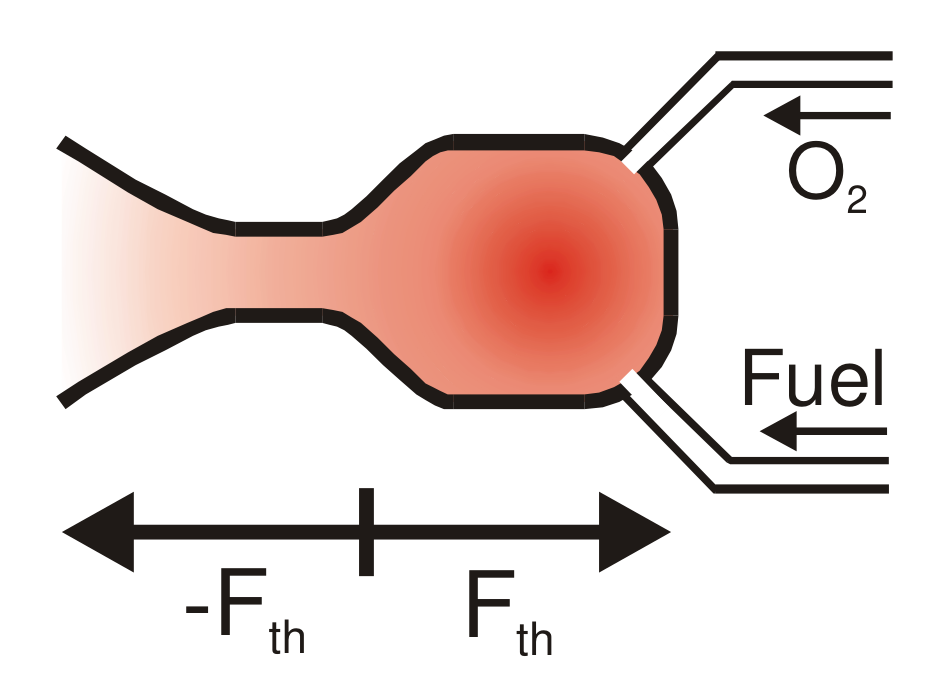
\includegraphics[width=0.5\hsize]{engine.png}
\end{figure}

\noindent
Sometimes the \textit{thrust-specific fuel consumption} (TSFC) is quoted in the literature. This is the amount of propellant that needs to be burned per second to obtain 1N of thrust. Thus the TSFC is the inverse of the Isp and has units of [$s \ m^{-1}$], or more intuitively [$kg \ s^{-1} N^{-1}$].\\
\\
\textbf{Note:} In Orbiter, the thrust is specified as a force, and has units of Newton [$1N = 1kg \ m \ s^{-2}$]. In the literature, thrust is often specified in units of kg. To convert such data into Orbiter units, multiply by $1g = 9.81 \ m \ s^{-2}$. Isp is specified as a velocity in Orbiter, with units of $m \ s^{-1}$. In the literature it is often given in units of seconds [s]. To convert to Orbiter units, again multiply by 1g.\\
\\
\textbf{How long will my fuel last?}\\
\\
The burn time $T_{b}$ at full thrust $F_{max}$ for fuel mass $m_{F}$ is given by

\[ T_{b} = \frac{m_{F} \ Isp}{F_{max}} \]

\noindent
\textbf{Pressure-dependent thrust efficiency}\\
\\
Most conventional rocket engines work less efficiently in the presence of ambient atmospheric pressure, because the ignited gas must be expelled through the nozzle against the outside pressure of the atmosphere. This leads to a reduction of the thrust force at ambient pressure \textit{p}:

\[ F(p) = F_{0} - p A \]

\noindent
where $F_{0}$ is the vacuum thrust rating and A has units of an area [$m^{2}$] and can be regarded as the \textit{effective nozzle cross section}. If we know the force $F_{1}$ generated at ambient pressure $p_{1}$, then

\[ F_{1} = F_{0} - p_{1}A \ \Rightarrow \ A = \frac{F_{0} - F_{1}}{p_{1}} \]

\noindent
and therefore

\[ F(p) = F_{0} - p\frac{F_{0} - F_{1}}{p_{1}} = F_{0}(1 - \frac{F_{0} - F_{1}}{F_{0}p_{1}}) = F_{0}(1 - p\eta) \]

\noindent
and likewise

\[ Isp(p) = Isp_{0}(1 - p\eta) \]

\noindent
In the literature, the pressure-dependency of engine thrust is often defined by specifying the Isp value for both vacuum and a given reference pressure (e.g. atmospheric pressure at sea level). Orbiter uses the same convention to apply pressure dependency.\\
\\
\textbf{Thrust level}\\
In Orbiter, thrusters can be driven at any level L between 0 (cutout) and 1 (full thrust). The actual thrust force generated by the engine is thus calculated as

\[ F(p) = F_{max}(p) \cdot L \]

\noindent
In reality, thrusters can often only be driven at maximum, or within a limited range below maximum. This is not currently implemented in Orbiter, but may be introduced in a future version.\\
\\
\textbf{Thruster placement and thrust direction}\\
\\
The effect of a thruster depends on its placement on the vessel, and the direction in which the thrust force is generated. In the most general case, a thruster will produce both a linear acceleration (due to a force) and an angular acceleration (do to torque).\\
Torque is generated if the force vector does not pass through the vessel’s centre of gravity (CG)

\begin{figure}[H]
  \centering
  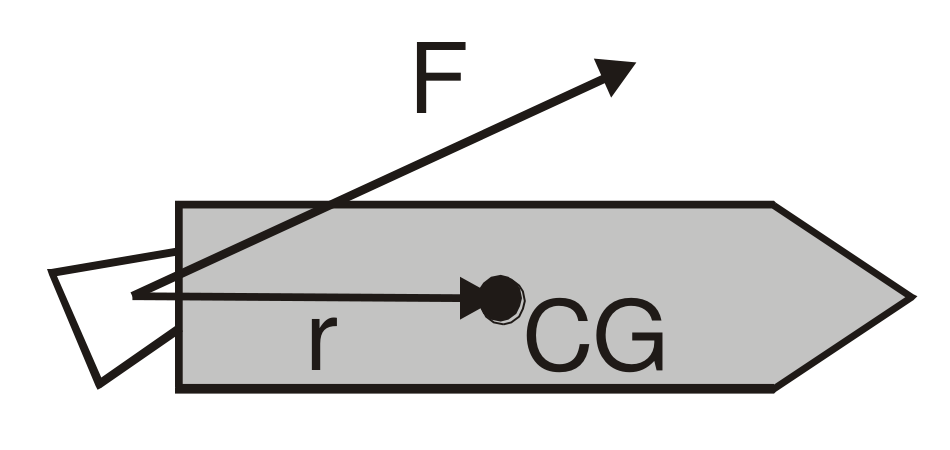
\includegraphics[width=0.5\hsize]{rocket_thrust.png}
\end{figure}

\noindent
The torque is then given by the cross product

\[ \vec{M} = \vec{F} \times \vec{r} \]

\noindent
(remember that Orbiter uses a left-handed coordinate system!) To avoid uncontrollable spin you should design your ship’s main engines so that their force vector passes through the CG. Vessel coordinates are always defined so that the CG is at the origin (0,0,0). Therefore, a thruster located at (0,0,-10) and generating thrust in direction (0,0,1) would not generate torque.\\
\\
\textbf{Attitude thrusters: Rotation}\\
\\
Sometimes generating torque is desired in order to rotate the spacecraft. For controlled attitude manouevres one then usually wants to change only the angular moment, without also inducing a linear acceleration. This requires the simultaneous operation of at least 2 thrusters so that their linear moments cancel.

\begin{figure}[H]
  \centering
  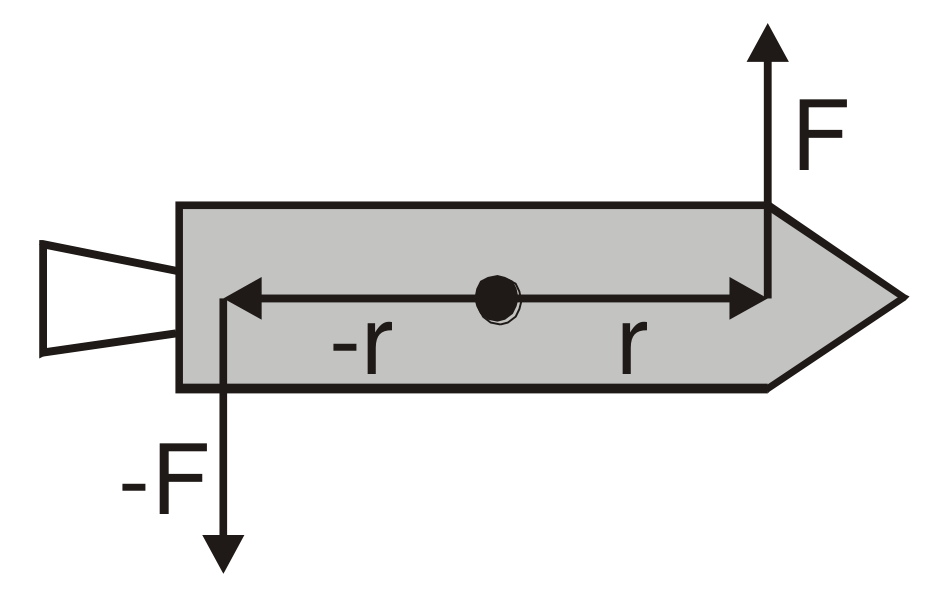
\includegraphics[width=0.5\hsize]{rocket_rotation.png}
\end{figure}

\noindent
\textbf{Attitude thrusters: Translation}\\
\\
In order to provide small linear accelerations in various directions (for example, to line the ship up with the docking port of a space station), thrusters must be driven single or in groups so that they don’t generate torque. Sometimes it is possible to re-use the rotational attitude thrusters for this task, but it is equally possible to add separate linear thrusters.\\

\begin{figure}[H]
  \centering
  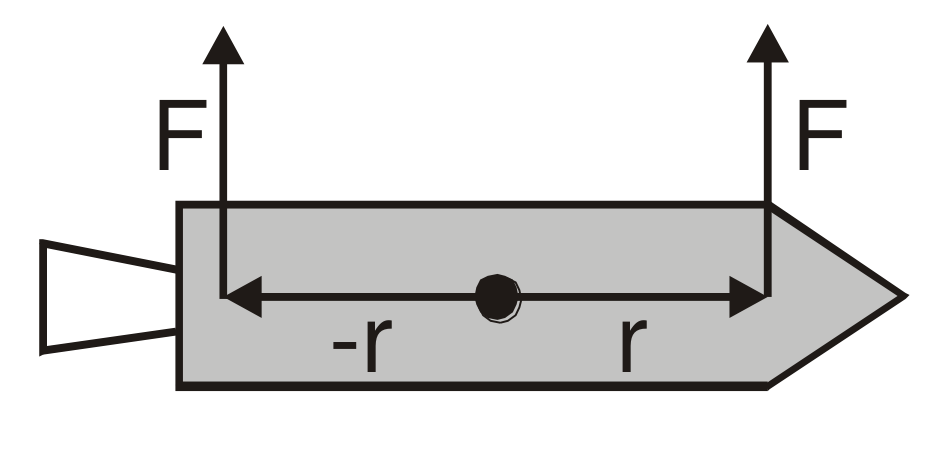
\includegraphics[width=0.5\hsize]{rocket_translation.png}
\end{figure}

\noindent
\textbf{Engine gimbal and thrust vectoring}\\
\\
Using attitude thrusters in a launch vehicle during the burn phase of the main engines is usually not practical. Instead, attitude control is performed by tilting the main engines and thereby generating a torque as described above. In practice this may be done by suspending the engines in a gimbal system which allows rotation around one or two axes. In Orbiter, this can be implemented by modifying the thrust direction of the engine.\\
\\
Another way to change the thrust direction is by inserting deflector plates into the exhaust stream.\\
\\
\textbf{Torque, angular momentum and angular velocity}\\
\\
The relationship between torque M and angular velocity is given by Euler’s equations for a rotating rigid body:
% TODO fix spacing between equations (2 and 3 show closer to each other than 1 and 2)
\[ J_{x}\dot{\omega}_{x} = M_{x} - (J_{z} - J_{y})\omega_{y}\omega_{z} \]
\[ J_{y}\dot{\omega}_{y} = M_{y} - (J_{x} - J_{z})\omega_{z}\omega_{x} \]
\[ J_{z}\dot{\omega}_{z} = M_{z} - (J_{y} - J_{x})\omega_{x}\omega_{y} \]

\noindent
where ($J_{x}$, $J_{y}$, $J_{z}$) are the principal moments of the inertia tensor (PMI), ($M_{x}$, $M_{y}$, $M_{z}$) are the components of the torque tensor, and ($\omega_{x}$, $\omega_{y}$, $\omega_{z}$) are the angular velocity components around the x, y, and z-axes. In Orbiter, this system of differential equations is solved by a trapezoid rule.


\subsubsection{Putting it all into the module}
Now that you know how thrusters work, it is time to add a few to your new ship. As with other vessel capabilities, thrusters should usually be designed in the \textit{clbkSetClassCaps} callback function, for example like this (assuming that \textit{MyVessel} is a class derived from \textit{VESSEL2}):

\begin{lstlisting}
void MyVessel::clbkSetClassCaps( FILEHANDLE cfg )
{
	// vessel caps definitions
}
\end{lstlisting}

\noindent
\textbf{Propellant resources}\\
\\
Thrusters can only be operated if they are connected to propellant resources (e.g. fuel tanks). To create a propellant resource:

\begin{lstlisting}
class MyVessel: public VESSEL
{
	...
	PROPELLANT_HANDLE ph_main;
}

void MyVessel::clbkSetClassCaps( FILEHANDLE cfg )
{
	...
	const double MAX_MAIN_FUEL = 1e5;
	ph_main = CreatePropellantResource( MAX_MAIN_FUEL );
	...
}
\end{lstlisting}

\noindent
which creates a fuel tank of capacity 10$^{5}$kg. \textit{CreatePropellantResource} returns a handle to the new tank, which is used later to connect thrusters to the tank.\\
\\
\textit{CreatePropellantResource} accepts two further optional parameters: the initial fuel mass, and a fuel efficiency factor \textit{eff} between 0 and 1. By default, the tank is full, with fuel efficiency 1. If an \textit{eff} < 1 is specified, then the thrust force generated by all connected thrusters is modified by

\[ F' = F \cdot eff \]

\noindent
\textbf{Creating thrusters}\\
\\
To add a new thruster, use the \textit{CreateThruster} command:
\begin{lstlisting}
class MyVessel: public VESSEL
{
	...
	THRUSTER_HANDLE th_main;
}

void MyVessel::clbkSetClassCaps( FILEHANDLE cfg )
{
	...
	const double MAX_MAIN_THRUST = 2e5;
	const double VAC_MAIN_ISP = 4200.0;
	th_main = CreateThruster( _V( 0, 0, -8 ), _V( 0, 0, 1 ),
		MAX_MAIN_THRUST, ph_main, VAC_MAIN_ISP );
	...
}
\end{lstlisting}

\noindent
This adds a thruster at position (0,0,-8) with a thrust vector in the positive z-direction, with the specified max. thrust and Isp values, and connected to the tank we added earlier. In this configuration, the engine efficiency is assumed not to be affected by atmospheric pressure. For increased realism, we could introduce pressure-dependency by adding an additional Isp value at a reference pressure, and the reference pressure itself:


\begin{lstlisting}
void MyVessel::clbkSetClassCaps( FILEHANDLE cfg )
{
	...
	const double MAX_MAIN_THRUST = 2e5;
	const double VAC_MAIN_ISP = 4200.0;
	const double NML_MAIN_ISP = 3500.0;
	const double P_NML = 101.4e3;
	th_main = CreateThruster( _V( 0, 0, -8 ), _V( 0, 0, 1 ),
		MAX_MAIN_THRUST, ph_main, VAC_MAIN_ISP, NML_MAIN_ISP, P_NML );
	...
}
\end{lstlisting}

\noindent
This reduces the Isp value at sea level to 3500 and performs a linear interpolation to obtain the Isp at arbitrary pressures. Note that we could have omitted the last parameter, \textit{P\_NML}, because the reference pressure defaults to 101.4 kPa (atmospheric pressure at Earth sea level).\\
\\
If you descend into a very dense planetary atmosphere, Orbiter will extrapolate the Isp value beyond sea level pressure, until Isp drops to zero. At this point, the thruster will stop working altogether.\\
\\
\textbf{Grouping thrusters}\\
\\
Although it is possible to address thrusters individually in your module, it is often easier to engage them in groups. Groups are also required to activate manual user thruster control via the keyboard or joystick, and the automatic navigation modes such as \textit{killrot}.\\
\\
% TODO fix overflow in following line
Orbiter has a number of standard thruster groups, such as \textit{THGROUP\_MAIN}, \textit{THGROUP\_RETRO}, \textit{THGROUP\_HOVER}, and a full set of attitude thruster groups. For a full listing, see \textit{VESSEL::CreateThrusterGroup} in the Reference Manual.\\
\\
It is the responsibility of the vessel designer to make sure that thrusters are grouped in a sensible way. For example, whenever the user presses the “+” key on the numerical keypad, all thrusters in \textit{THGROUP\_MAIN} will fire. If the thrusters grouped in \textit{THGROUP\_MAIN} behave in an unexpected or non-intuitive way it will be confusing to the user. Furthermore, if attitude thrusters are not appropriately grouped, some or all of the navigation modes may fail.\\
\\
To group thrusters, use the \textit{CreateThrusterGroup} command:

\begin{lstlisting}
void MyVessel::clbkSetClassCaps( FILEHANDLE cfg )
{
	...
	thg_main = CreateThrusterGroup( th_main, 2, THGROUP_MAIN );
	...
}
\end{lstlisting}

\noindent
(this assumes that \textit{th\_main} is an array of 2 thruster handles which have been created previously). The function returns a handle to the group which can be used later to address the group.\\
\\
Apart from the standard groups, Orbiter allows to create custom groups by using the \textit{THGROUP\_USER} label. Custom groups are not engaged by any of the standard manual or automatic control methods, therefore the module must implement a suitable control interface for these groups.


\subsubsection{Defining exhaust flames}
When you define a thruster with \textit{CreateThruster}, Orbiter will not automatically generate visuals for the exhaust flames when the thruster is engaged. Sometimes exhaust flames may not be appropriate, or, more importantly, you may want to detach the \textit{logical} thruster definition from the physical definition (more about this below).\\
\\
To create an exhaust flame definition use the \textit{AddExhaust} function. \textit{AddExhaust} comes in two flavours:
\begin{itemize}
\item \textit{UINT AddExhaust( THRUSTER\_HANDLE th, double lscale, double wscale, SURFHANDLE tex = 0 ) const}
\item \textit{UINT AddExhaust( THRUSTER\_HANDLE th, double lscale, double wscale, const VECTOR3 \&pos, const VECTOR3 \&dir, SURFHANDLE tex = 0 ) const}
\end{itemize}

\noindent
Both versions require a handle to the logical thruster they are linked to, and two size parameters (longitudinal and transversal scaling), but while the first version takes exhaust location and direction directly from the thruster definition, the second version gets location and direction passed as parameters.\\
\\
Here is an example demonstrating how you would use the second version of \textit{AddExhaust}:\\
\\
Let’s assume you build a rocket propelled by 4 main engines arranged in a regular square pattern. The engines have fixed orientation (no individual gimbal mode) and all thrust force vectors are parallel. In addition, the engines produce identical thrust magnitudes at all times.\\
\\
Then the 4 engines can be represented by a single logical thruster, whose magnitude is the sum of the 4 actual engines, and positioned in the geometric centre. This simplifies the code, and is more efficient, because Orbiter does not need to add up 4 individual force vectors.\\
\\
However, you still want to see exhaust flames for each of the 4 engines, so you would use the second version of \textit{AddExhaust} to define 4 exhaust flames at the correct positions.\\
\\
The disadvantage of the second version is that changes in the position or orientation of the thruster (for example as a result of \textit{SetThrusterPos} or \textit{SetThrusterDir}) are not automatically propagated to the exhaust flames. Therefore, if you plan to move or tilt the thrusters, you should create them individually and use the first version of \textit{AddExhaust}.\\
\\
\textbf{Custom exhaust textures}\\
\\
By default, Orbiter uses a standard texture to render exhaust flames. If you want to customise the exhaust appearance on a per-thruster basis, you can pass a nonzero surface handle tex to both of the \textit{AddExhaust} versions. To obtain a surface handle for a custom texture, use the \textit{oapiRegisterExhaustTexture} function.

\begin{lstlisting}
...
SURFHANDLE tex = oapiRegisterExhaustTexture( "MyExhaust" );
AddExhaust( th_main, 10, 2, tex );
...
\end{lstlisting}

\noindent
The texture file must be stored in DDS format in Orbiter’s default texture directory. Note that \textit{oapiRegisterExhaustTexture} can be safely called multiple times with the same texture.


\subsection{Air-breathing engines}
Orbiter is not limited to rocket engines. Other devices for generating thrust can be implemented as well, from turbojet engines to solar sails or some hypothetical future technology. Unlike conventional rocket engines, which are natively supported by the Orbiter core, custom designs require a bit more work from the developer. As an example, I will here discuss the (tentative) scramjet engine implementation used by the delta-glider.\\
\\
A ramjet engine is a type of a jet engine which compresses the air for combustion not by any mechanical rotating machinery, but simply by “ramming” through the atmosphere, i.e. by using the aircraft’s velocity in the airstream. This is an efficient way of generating thrust at supersonic speeds, but does not work at very low speed. (A scramjet is a variant where the air is not slowed down to subsonic speeds in the combustor and therefore avoids excessive heating at extreme velocities).\\
\\
A typical ramjet engine is composed of 3 sections:

\begin{itemize}
\item the inlet diffuser where the air is isentropically decelerated, with pressure increasing from freestream pressure $p_{\infty}$ to $p_{d}$, and temperature increasing from freestream temperature $T_{\infty}$ to $T_{d}$.
\item the combustion chamber, where the air-fuel mixture is burned at constant pressure $p_{b} = p_{d}$, and temperature increases from $T_{d}$ to $T_{b}$.
\item the exhaust nozzle, where the hot, high-pressure gas is expanded isentropically, with pressure decreasing from $p_{b}$ to $p_{\infty}$, and temperature decreasing from $T_{b}$ to $T_{e}$.
\end{itemize}

\noindent
The temperatures and pressures in the three parts of the engine (diffuser, burner and exhaust) can be calculated in the following form:

%TODO place equations into columns
\[ T_{d} = T_{\infty}\left(1 + \frac{\gamma - 1}{2} M_{\infty}^{2}\right) \]
\[ T_{b} = max(T_{b0},T_{d}) \]
\[ T_{e} = T_{b}\left(\frac{p_{e}}{p_{b}}\right)^{(\gamma - 1) / \gamma} \]
\[ p_{d} = p_{\infty}\left(\frac{T_{d}}{T_{\infty}}\right)^{\gamma / (\gamma - 1)} \]
\[ p_{b} = p_{d} \]
\[ p_{e} = p_{\infty} \]

\noindent
where $M_{\infty}$ is the freestream Mach number, $\gamma$ is the ratio of specific heats, and $T_{b0}$ is the burner temperature limit, an engine design parameter defined by the heat resistance of the combustion chamber material. Note that if at high velocities $T_{d} > T_{b0}$, the engine will start to overheat purely from the isentropic compression in the diffuser, without any combustion taking place! The figure below shows an example for the temperature distribution in the engine compartments as a function of freestream Mach number. The example assumes a burner temperature limit of $T_{b0}$ = 3200 K. In this case, the limiting velocity is $v$ = Mach 8.2.

\begin{figure}[H]
  \centering
  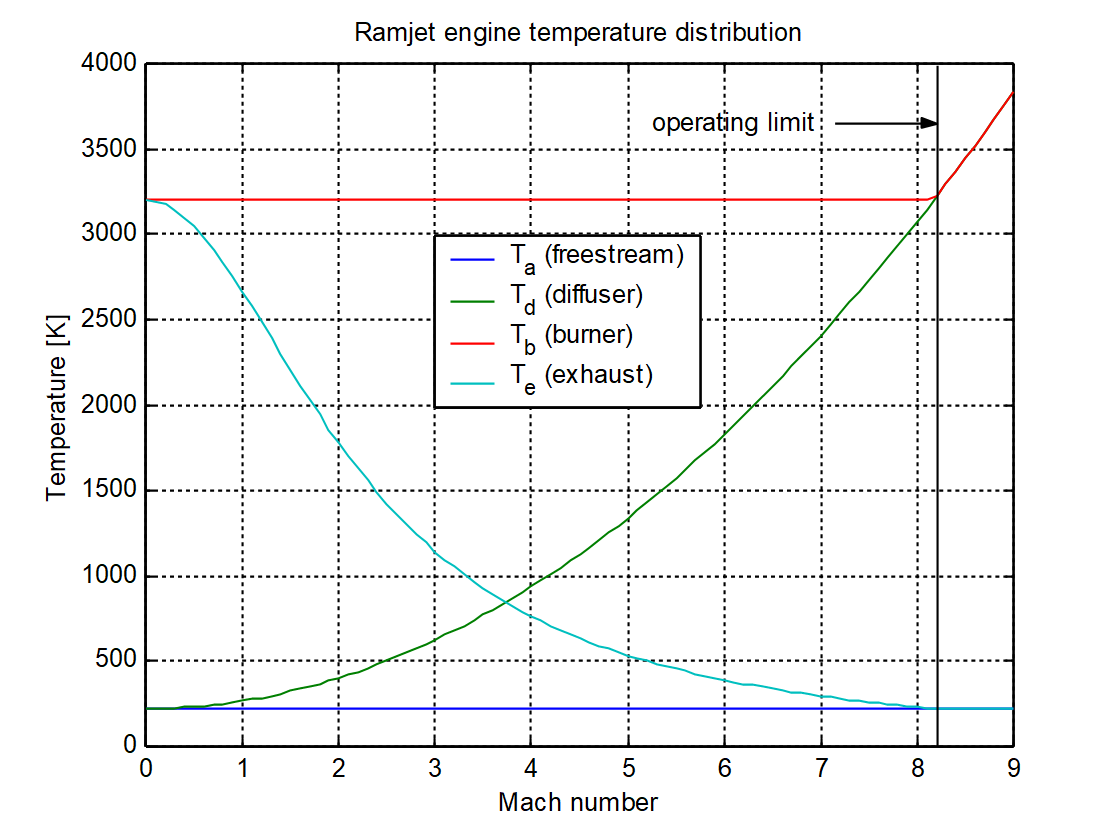
\includegraphics[width=0.5\hsize]{ramjet_temp.png}
\end{figure}

\noindent
To calculate the thrust generated by a scramjet, we start from the fundamental thrust equation for jet propulsion,

\[ F = (\dot{m}_{a} + \dot{m}_{f})v_{e} - \dot{m}_{a} v_{\infty} + (p_{e} - p_{\infty})A_{e} \]

\noindent
where $\dot{m}_{a}$ and $\dot{m}_{f}$ are the air and fuel mass rates, respectively (using the common notation $\dot{x} = dx / dt$), $v_{e}$ and $v_{\infty}$ are the exhaust and freestream velocities, and $A_{e}$ is the exhaust cross section.\\
\\
Because of the assumption $p_{e} = p_{\infty}$ the last term vanishes. The \textit{specific thrust} is then given by

\[ \frac{F}{\dot{m}_{a}} = (1 + D)v_{e} - v_{\infty} \]

\noindent
where $D = \dot{m}_{f} / \dot{m}_{a}$ is the \textit{fuel-to-air} ratio.\\
\\
The amount of fuel burned in the combustion chamber must be adjusted so that the burner temperature limit is not exceeded. This leads to the following expression for \textit{D}:

\[ D = \frac{T_{b} - T_{d}}{Q / c_{p} - T_{b}} \]

\noindent
where \textit{Q} is a fuel-specific heating value and $c_{p}$ is the specific heat at constant pressure, given by

\[ c_{P} = \frac{\gamma R}{\gamma - 1} \]

\noindent
The mass flow of air collected by the engine is a function of air intake cross section $A_{i}$, freestream density $\rho_{\infty}$ and freestream velocity $v_{\infty}$:

\[ \dot{m}_{a} = \rho_{\infty} v_{\infty} A_{i} \]

\noindent
where $v_{\infty}$ can be expressed in terms of the freestream Mach number:

\[ v_{\infty} = M_{\infty} \sqrt{\gamma R T_{\infty}} \]

\noindent
From the above equations for \textit{D} and $\dot{m}_{a}$ we can calculate the fuel rate $\dot{m}_{f}$ required to achieve combustion temperature $T_{b}$.\\
\\
The final quantity required to calculate \textit{F} is the exhaust velocity $v_{e}$. This can be obtained from the energy balance

\[ c_{p} T_{b} = c_{p} T_{e} + v^{2}_{e} / 2 \]

\noindent
We now have all the components to calculate the thrust \textit{F} generated by the engine. The graphs below show various scramjet parameters for velocities in the range from Mach 0 to Mach 10 at an altitude of 10 km (assuming $\rho_{\infty}$ = 0.43 kg/m$^{3}$ and $T_{\infty}$ = 225 K). The DG engine design parameters in this example are \textit{Q} = 4.5 $\cdot$ 10$^{7}$ J/kg, $A_{i}$ = 0.6 m$^{2}$, and $T_{b0}$ = 3200 K.

\begin{figure}[H]
	\centering
	\subfigure{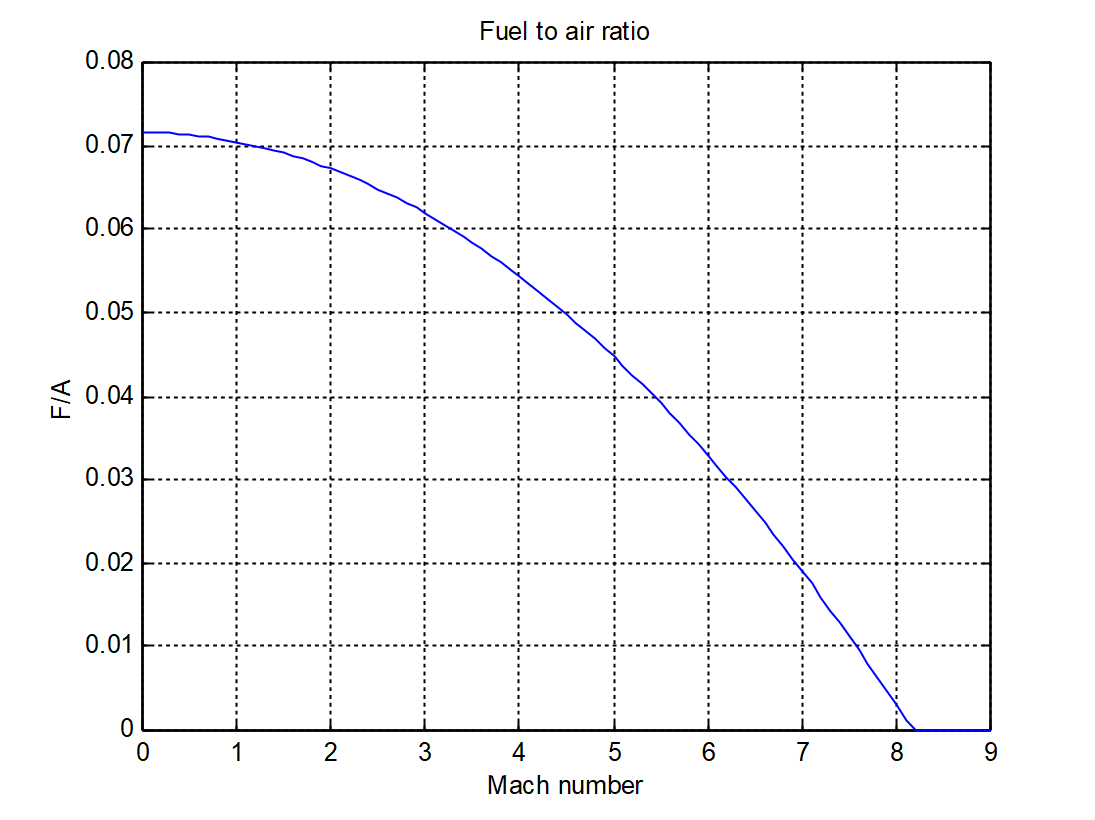
\includegraphics[width=0.49\textwidth]{fuel_to_air_ratio.png}}
	\subfigure{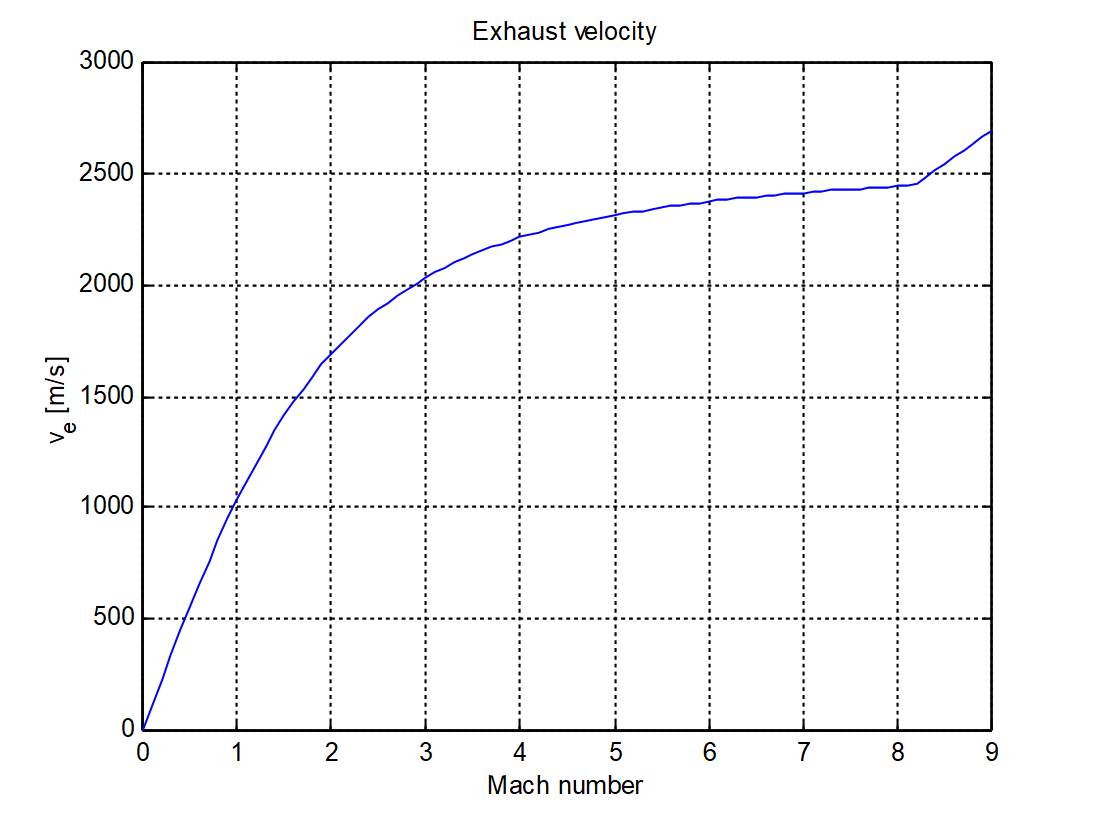
\includegraphics[width=0.49\textwidth]{enhaust_velocity.png}}
	\subfigure{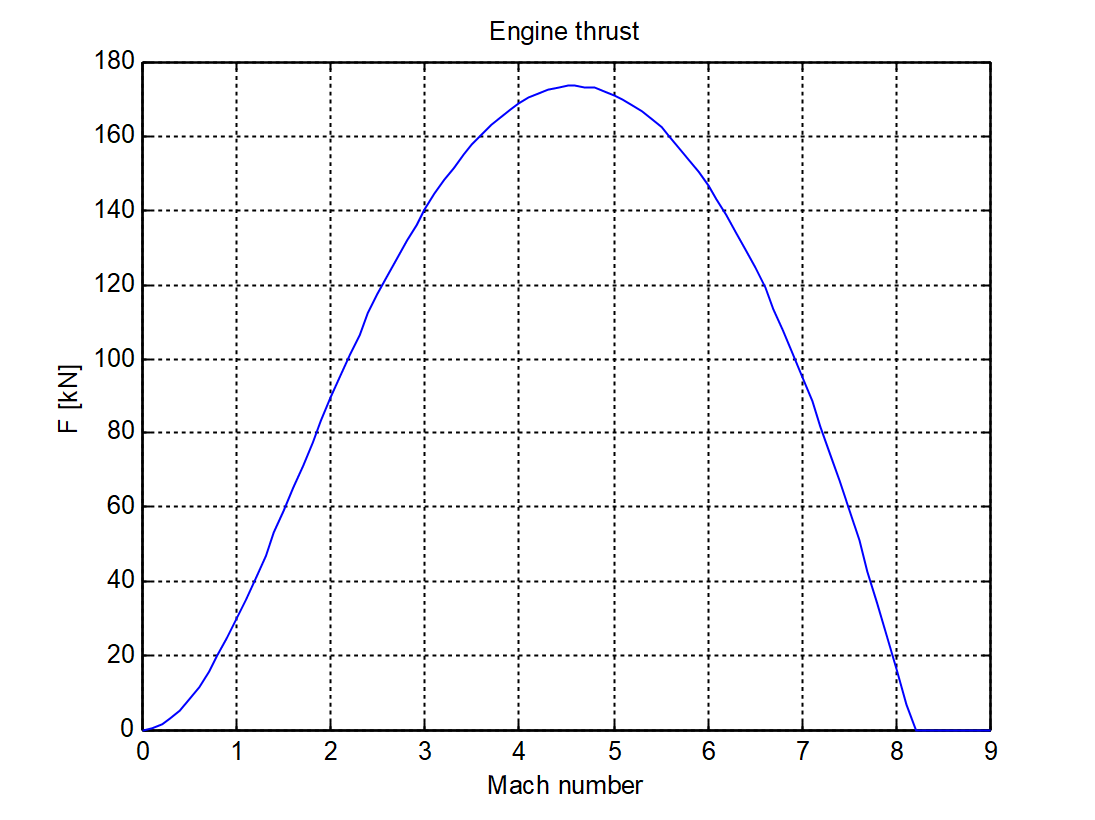
\includegraphics[width=0.49\textwidth]{engine_thrust.png}}
	\subfigure{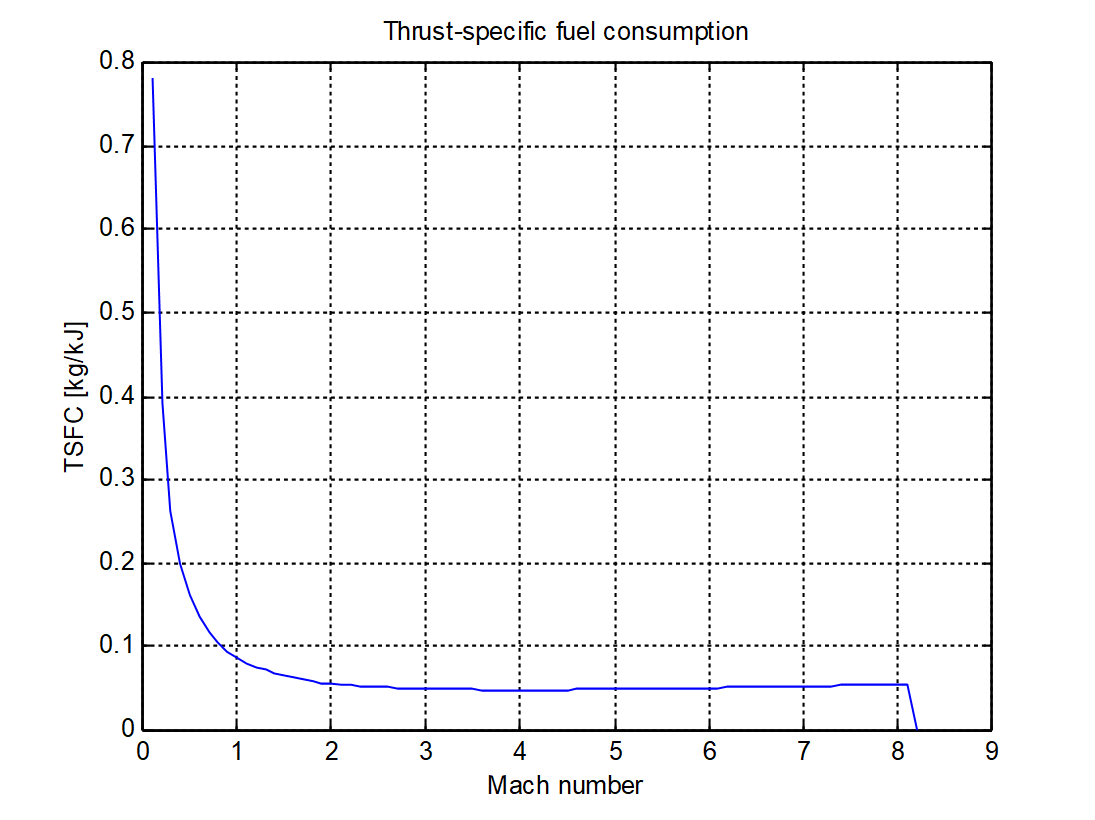
\includegraphics[width=0.49\textwidth]{thrust_specific_fuel_consumption.png}}
\end{figure}


\subsection{Rendering re-entry flames}
To visualise the friction heat dissipation during atmospheric reentry, Orbiter supports the rendering of “re-entry flames”. To calculate the amount of heat generated per surface area and time (and to scale the exhaust flames) Orbiter uses this formula:

\[ P = \frac{1}{2} \rho v^{3} \]

\noindent
where $\rho$ is the atmospheric density, and \textit{v} is the vessel’s airspeed. Orbiter renders exhaust flames if $P > P_{0}$ where $P_{0}$ is a user defined limit. The size and opacity of the reentry flames is scaled by

\[ s = min\left(1,\frac{P - P_{0}}{5P_{0}}\right) \]

\noindent
In addition, the user can specify scaling factors for length and width of the reentry texture, as well as the texture itself.\\
\\
Orbiter by default uses its own texture to render reentry flames. If you want to change the texture globally, you need to replace reentry.dds in the Textures subdirectory. If you only want to modify the texture for a specific vessel class, you need to load a custom texture, and then set your render options:

\begin{lstlisting}
void MyVessel::clbkSetClassCaps( FILEHANDLE cfg )
{
	...
	SURFHANDLE tex = oapiRegisterReentryTexture( "MyReentryFlame" );
	SetReentryTexture( tex, my_plimit, my_lscale, my_wscale );
	...
}
\end{lstlisting}

\noindent
Reentry textures require a specific layout. They consist of an elongated part in the left half of the texture map, and a circular part in the upper right corner. The lower right corner is not currently used. This is how the alpha channel of the default reentry.dds looks like:

\begin{figure}[H]
  \centering
  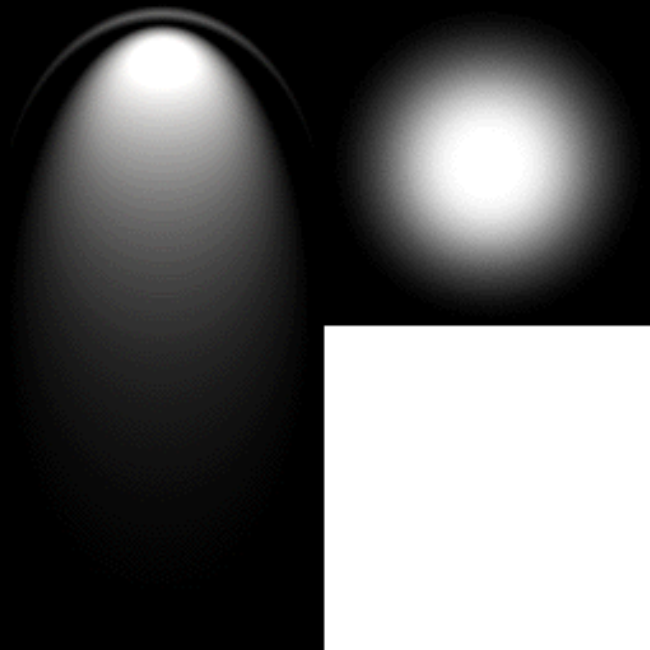
\includegraphics[width=0.5\hsize]{reentry_dds.png}
\end{figure}

\noindent
Note that Orbiter automatically adds a colour component to the texture depending on the value of \textit{s}, from red to white. If this is sufficient for your custom reentry flame, leave the RGB channels of the texture pure white. Otherwise you may want to experiment with additional texture colours.\\
\\
If you want to suppress rendering of reentry flames for your vessel altogether, use

\begin{lstlisting}
...
SetReentryTexture( NULL );
...
\end{lstlisting}


\subsection{Adding particle streams for exhaust and reentry effects}
Orbiter supports particle streams for rendering contrails, exhaust gases, reentry plasma trails etc. Particle streams consist of a series of textured “billboard” objects which always face the camera. The streams can be customised with a set of parameters and allow the simulation of a variety of effects.\\
\\
\textbf{The PARTICLESTREAMSPEC structure}\\
\\
At creation, the particle stream can be customised by passing a \textit{PARTICLESTREAMSPEC} structure to \textit{VESSEL::AddExhaustStream} and \textit{VESSEL::AddReentryStream}. The structure is defined as follows:

\begin{lstlisting}
typedef struct
{
	DWORD flags;
	double srcsize;
	double srcrate;
	double v0;
	double srcspread;
	double lifetime;
	double growthrate;
	double atmslowdown;
	enum LTYPE { EMISSIVE, DIFFUSE } ltype;
	enum LEVELMAP { LVL_FLAT, LVL_LIN, LVL_SQRT,
		LVL_PLIN, LVL_PSQRT } levelmap;
	double lmin, lmax;
	enum ATMSMAP { ATM_FLAT, ATM_PLIN } atmsmap;
	double amin, amax;
	SURFHANDLE tex;
} PARTICLESTREAMSPEC;
\end{lstlisting}

\noindent
\textit{srcrate}
\begin{adjustwidth}{1cm}{0cm}
The (average) rate at which particles are created by the emission source [Hz].
\\
\end{adjustwidth}


\noindent
\textit{v0}
\begin{adjustwidth}{1cm}{0cm}
The (average) emission velocity of particles by the emission source [m/s]
\\
\end{adjustwidth}

\noindent
\textit{ltype}
\begin{adjustwidth}{1cm}{0cm}
Defines the material lighting method when rendering the particles.

\begin{itemize}
\item EMISSIVE: Particles are rendered emissive (self-radiating). This is appropriate for streams representing ionized exhaust gases, or plasma streams during reentry.
\item DIFFUSE: Particles are rendered diffuse (diffuse reflection of external light sources). This is appropriate for smoke and vapour trails.
\end{itemize}
\end{adjustwidth}

\noindent
\textit{levelmap}
\begin{adjustwidth}{1cm}{0cm}
Defines the mapping between the level parameter $L$ (e.g. thruster level) and the alpha value $\alpha$ (opacity) of the generated particle. The higher the alpha value, the more solid the stream will appear. This parameter is only used for exhaust streams. The following options are available:

\begin{itemize}
\item LVL\_FLAT: constant mapping, i.e. alpha is independent of th reference level: $\alpha = lmin$
\item LVL\_LIN: linear mapping: $\alpha = L$
\item LVL\_SQRT: square root mapping: $\alpha = \sqrt{L}$
\item LVL\_PLIN: linear mapping in sub-range: $\alpha = 
\left\{
\begin{array}{ll}
	0 & L < lmin \\
	\frac{L - lmin}{lmax - lmin} & lmin \leq L \leq lmax \\
	1 & L > lmax \\
\end{array} 
\right. $
\item LVL\_PSQRT: square root mapping in sub-range: $\alpha =
\left\{
\begin{array}{ll}
	0 & L < lmin \\
	\sqrt{\frac{L - lmin}{lmax - lmin}} & lmin \leq L \leq lmax \\
	1 & L > lmax \\
\end{array} 
\right. $
\end{itemize}
\end{adjustwidth}

\noindent
\textit{lmin, lmax}
\begin{adjustwidth}{1cm}{0cm}
Defines min and max levels for alpha mapping. Only used if \textit{levelmap} is \textit{CONST}, \textit{PLIN} or \textit{PSQRT} (see above). For \textit{CONST}, only $lmin$ is used. For \textit{PLIN} and \textit{PSQRT}, $lmin < lmax$ is required. Note that $lmin < 0$ is valid – this will cause the stream to produce particles even when the reference level is 0. Likewise, $lmax > 1$ is valid – this will cause the alpha value of the particles to remain < 1 even at reference level 1.
\\
\end{adjustwidth}

\noindent
\textit{atmsmap}
\begin{adjustwidth}{1cm}{0cm}
Defines the mapping between atmospheric parameters and the alpha value $\alpha$ (opacity) of the generated particle. The following options are available:

\begin{itemize}
\item ATM\_FLAT: constant mapping, i.e. alpha is independent of atmospheric parameters: $\alpha = amin$
\item ATM\_PLIN: linear mapping of ambient atmospheric parameter $x$:\\
$\alpha = 
\left\{
\begin{array}{ll}
	0 & x < amin \\
	\frac{x - amin}{amax - amin} & amin \leq x \leq amax \\
	1 & x > amax \\
\end{array} 
\right. $
\item ATM\_PLOG: logarithmic mapping of ambient atmospheric parameter $x$:\\
$\alpha = 
\left\{
\begin{array}{ll}
	0 & x < amin \\
	\frac{ln(x / amin)}{ln(amax / amin)} & amin \leq x \leq amax \\
	1 & x > amax \\
\end{array} 
\right. $
\end{itemize}
For exhaust streams, atmospheric parameter $x$ is the ambient atmospheric density, $\rho$. For reentry streams, $x$ is defined as $x = \frac{1}{2}\rho v^{3}$ ($v$: airspeed) which is proportional to the friction power in turbulent airflow (omitting geometry-related parameters).\\
\\
\end{adjustwidth}

\noindent
\textit{amin, amax}
\begin{adjustwidth}{1cm}{0cm}
Defines min and max atmospheric parameter (ambient density or friction power) for alpha mapping. $amin < amax$ is required. For \textit{PLIN}, $amin < 0$ is admissible to enable particle generation at zero density. For \textit{PLOG}, $amin > 0$ is required. 

\begin{figure}[H]
	\centering
	\subfigure{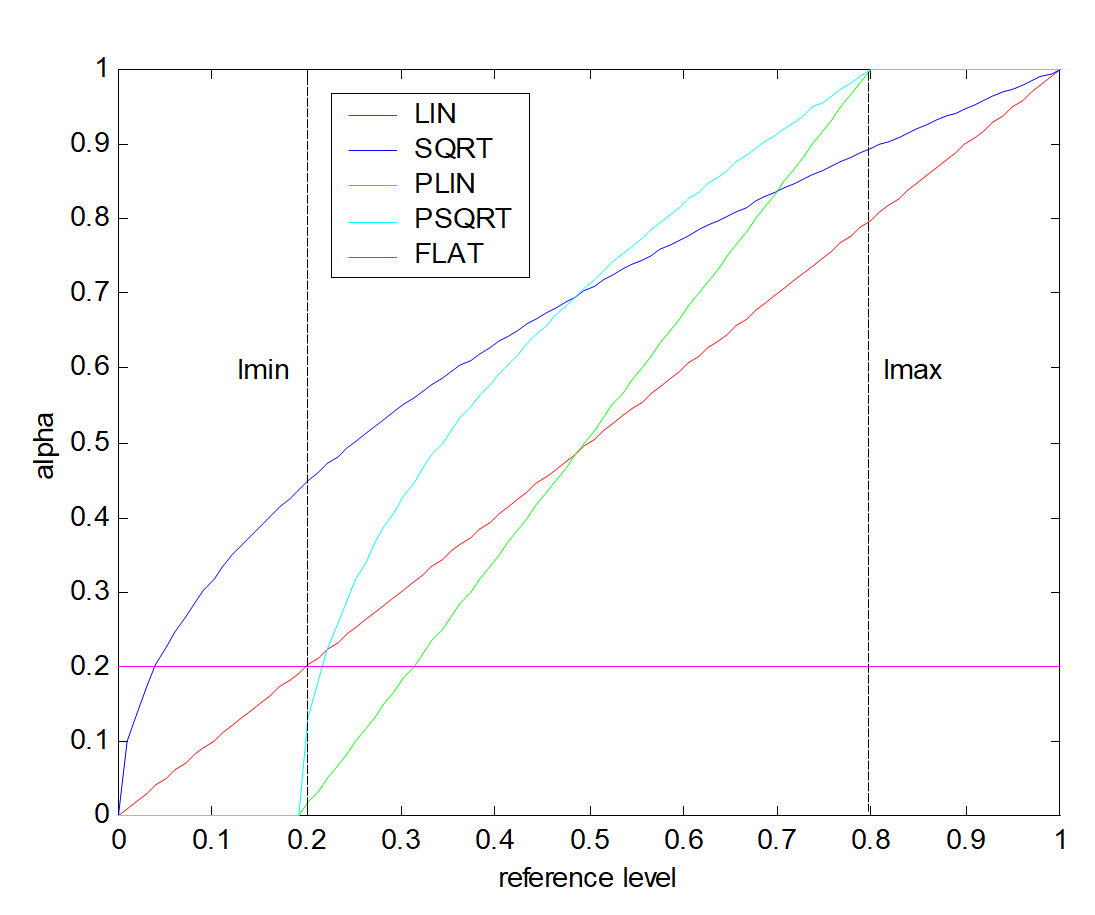
\includegraphics[width=0.49\textwidth]{particle_level.png}}
	\subfigure{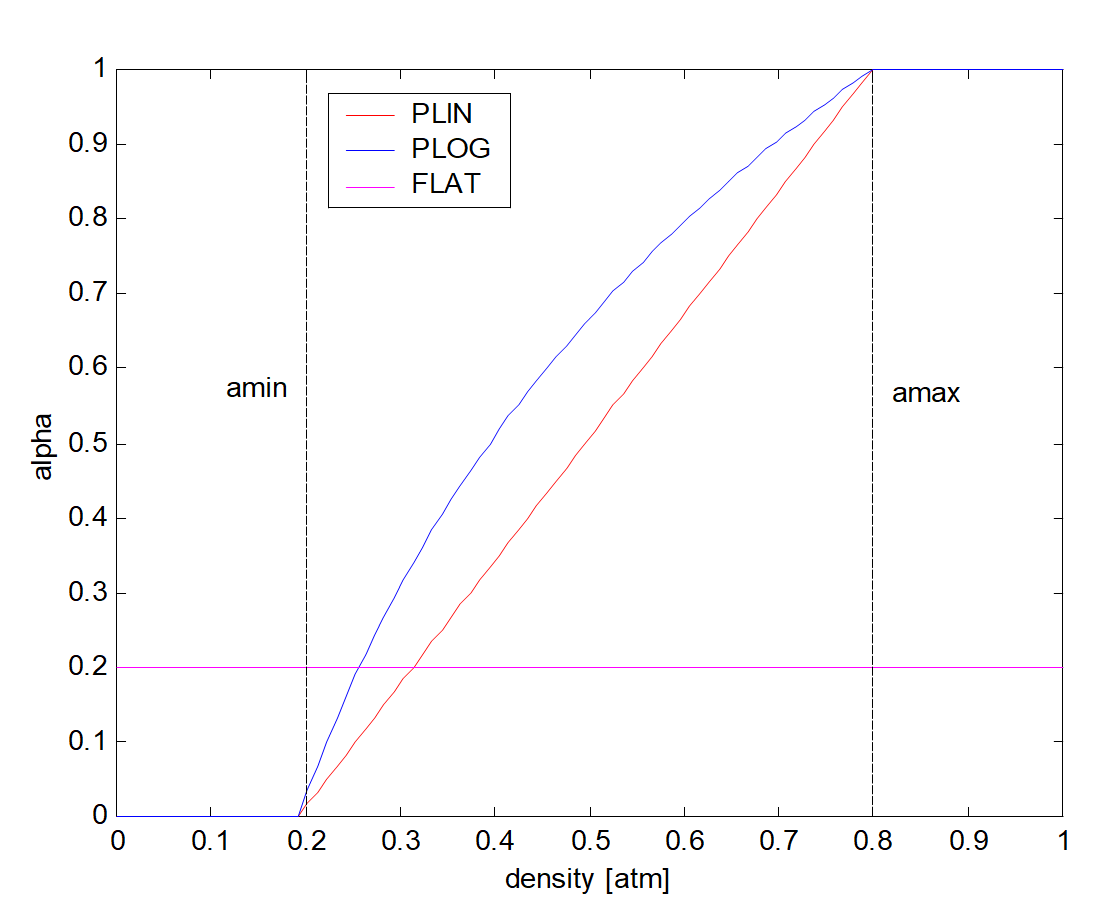
\includegraphics[width=0.49\textwidth]{particle_atmosphere.png}}
	\caption{The particle alpha value as a function of reference level (left) and atmospheric parameter (right) for different ‘levelmap’ and ‘atmsmap’ modes.}
\end{figure}
\end{adjustwidth}


\subsection{Atmospheric flight model}
\subsubsection{Lift and drag theory}
Drag is a force acting on the vessel in the direction of the freestream airflow. It is composed from several components:
\begin{enumerate}
\item The \textit{skin friction drag} caused by the boundary layer surrounding the airfoil.
\item The \textit{pressure drag} caused by separation of flow from the surface.
\item The \textit{wave drag} at supersonic velocities.
\item \textit{Induced drag}, caused by airflow around the wingtip (finite wing) from the lower to the upper surface.
\end{enumerate}
\noindent
The combination of components 1-3 is defined as \textit{profile drag} or \textit{parasite drag}.\\
\\
Lift is an upward force (perpendicular to the airflow) caused by the shape of the airfoil and its orientation to the airflow.\\
\\
Drag $D$ and lift $L$ of an airfoil are expressed by the drag and lift coefficients $c_{D}$ and $c_{L}$, with

\[ c_{D} = \frac{D}{q_{\infty} S} \]
\[ c_{L} = \frac{L}{q_{\infty} S} \]

\noindent
where $q_{\infty} = 1/2 \rho_{\infty} V^{2}_{\infty}$ is the freestream dynamic pressure, and $S$ is the wing area. Generally, $c_{D}$ and $c_{L}$, will be functions of the angle of attack, the Mach number, and the Reynolds number. We now split $c_{D}$ in the components of profile and induced drag. Induced drag is a result of lift and can be expressed as a function of $c_{L}$:

\[ c_{D} = c_{D,e} + \frac{c_{L}^{2}}{\pi eA} \]

\noindent
where $e$ is a span efficiency factor, and $A$ is the wing aspect ratio, defined as $b^{2}/S$ with wing span $b$.\\
\\
The profile component $c_{D,e}$ will change with angle of attack. We assume that $c_{D,e}$ can be expressed as the combination of a zero-lift component $c_{D,0}$ and a component depending on $c_{L}$:

\[ c_{D,e} = c_{D,0} + rc_{L}^{2} \]

\noindent
Here, $r$ is a form constant which is usually determined empirically. We can now incorporate the lift-dependent term of $c_{D,e}$ into the factor $e$, to give

\[ c_{D} = c_{D,0} + \frac{c_{L}^{2}}{\pi eA} \]

\noindent
where $\varepsilon = e / (r \pi eA + 1)$ is the \textit{Oswald efficiency factor}.\\
\\
When implementing an airfoil in Orbiter, the user must supply a function which calculates $c_{L}$ and $c_{D}$ for a given set of parameters (angle of attack, Mach number and Reynolds number). Orbiter provides a helper function (oapiGetInducedDrag) to calculate the induced drag component with the above formula.


\subsubsection{Lift and drag in transonic and supersonic flight}
(to be completed)


\subsubsection{Angular moments and vessel stability}
(to be completed)


\subsubsection{Angular drag}
Similar to (linear) drag which produces a force acting against a vessel’s airspeed vector, a rotating vessel will experience angular drag which acts against the angular velocity, thus slowing the rotation. Orbiter uses the following formulae to calculate angular damping:

\[ dM_{x} = -q'S_{y}c_{\alpha,x}\omega_{x} \]
\[ dM_{y} = -q'S_{y}c_{\alpha,y}\omega_{y} \]
\[ dM_{z} = -q'S_{y}c_{\alpha,z}\omega_{z} \]

\noindent
where $q' = 1/2 \rho_{\infty}(V_{\infty} + V_{0})^{2}$ is a modified dynamic pressure which ensures that angular drag also occurs at low airspeeds (Orbiter currently uses a fixed $V_{0}$ = 30 m/s). $S_{y}$ is the vessel’s cross section projected along the vertical (y) axis, used as a reference area. $S_{y}$ is the y-component of the vector passed to \textit{VESSEL::SetCrossSections()}. $c_{\alpha,x}$, $c_{\alpha,y}$ and $c_{\alpha,z}$ are the drag coefficients for rotations around the $x$, $y$, and $z$ vessel axes as defined by \textit{VESSEL::SetRotDrag()}. $\omega_{x}$, $\omega_{y}$ and $\omega_{z}$ are the angular velocities around the vessel axes, and $dM_{x}$, $dM_{y}$ and $dM_{z}$ are the changes in torque due to damping.\\
\\
Angular drag is determined by the vessel shape. Developers can adjust the effect of angular damping in the atmosphere by adjusting the coefficients passed to \textit{VESSEL::SetRotDrag()}. Higher coefficients make a vessel less responsive to control input, and reduce oscillations around equilibrium orientation.



\subsubsection{API interface for airfoil definition}
% TODO text overflow
To define the lift and drag characteristics for a spacecraft in the DLL module, use the \textit{VESSEL::CreateAirfoil} method. An airfoil is defined as a cross section through a wing. In Orbiter, we use the term airfoil for any components of the vessel which produce lift and/or drag forces. Multiple airfoils can be defined for a single vessel (for example for the left and right wing, the body, the horizontal and vertical stabilizers in the tail, etc.). It is usually best to keep the number of airfoils low to keep the flight model predictable and to improve simulation performance.\\
\\
Orbiter distinguishes two different types of airfoil orientations: airfoils which create vertical lift (e.g. wings) and airfoils which create horizontal “lift”, e.g. vertical stabilisers. Even vessels without any wings or other aerodynamic surfaces should define at least one horizontal and one vertical airfoil to define their atmospheric drag behaviour (even blunt objects such as reentry capsules which have no similarity to an aircraft produce drag and lift forces).\\
\\
When calling the \textit{CreateAirfoil} method, the user must provide
\begin{itemize}
\item basic airfoil parameters (orientation, wing area, chord length and wing aspect ratio).
\item the force attack point (i.e. the point on the vessel on which the lift and drag forces for this airfoil act). This influences the angular moments generated by the forces.
\item a callback function which calculates the lift, drag and moment coefficients of the airfoil as a function of angle of attack $\alpha$, Mach number $M$ and Reynolds number $Re$.
\end{itemize}

\noindent
The coefficients decide how much lift and drag is generated by the airfoil. The lift and drag forces ($L$ and $D$) are obtained from the moments ($c_{L}$ and $c_{D}$) by

\[ L(\alpha,M,Re) = c_{L}(\alpha,M,Re)q_{\infty}S \]
\[ D(\alpha,M,Re) = c_{D}(\alpha,M,Re)q_{\infty}S \]

\noindent
with freestream dynamic pressure $q_{\infty} = 1/2\rho v^{2}$, and reference area $S$. The function which calculates $c_{L}$ and $c_{D}$ must be able to handle arbitrary angles of attack ($-\pi$ to $\pi$) and very high Mach numbers which may occur during LEO insertion and atmospheric entry (orbital velocity for a low Earth orbit is equivalent to $M$ > 20!)\\
\\
The Reynolds number is a parameter dependent on atmospheric viscosity $\mu$:

\[ Re = \frac{\rho vc}{\mu} \]

\noindent
with freestream airspeed $v$ and density $\rho$. In the current Orbiter version, $\mu$ is assumed constant ($\mu$ = 1.6894$\cdot$10$^{-5}$ kg m-1 s-1). In future versions, $\mu$ will depend on the atmospheric composition and temperature.\\
\\
The direction of the lift force vector is defined in Orbiter as

\[ \hat{L}_{\alpha} = (0,-v_{z},v_{y}) / \sqrt{v_{y}^{2} + v_{z}^{2}} \]
\[ \hat{L}_{\beta} = (-v_{z},0,v_{x}) / \sqrt{v_{x}^{2} + v_{z}^{2}} \]

\noindent
for vertical and horizontal lift components, respectively, where ($v_{x}$,$v_{y}$,$v_{z}$) is the freestream airflow vector in vessel coordinates. This means that $\hat{L}_{\alpha}$ is rotated 90° counter-clockwise against the projection of the airflow vector into the yz-plane, and $\hat{L}_{\beta}$ is rotated 90° counter-clockwise against the projection of the airflow vector into the xz-plane. Since $\alpha$ and $\beta$ are defined as

\[ \alpha = arctan(v_{y} / -v_{z}) \]
\[ \beta = arctan(v_{x} / -v_{z}) \]

\noindent
we find the following relations between $\alpha$ or $\beta$ and the direction of lift:

\begin{table}[H]
	\centering
	\begin{tabular}{ |c|c| }
	\hline\rule{0pt}{2ex}
	\textbf{$\alpha$} & \textbf{lift direction} \\
	\hline\rule{0pt}{2ex}
	0º & up (+y)\\
	\hline\rule{0pt}{2ex}
	90º & forward (+z)\\
	\hline\rule{0pt}{2ex}
	180º & down (-y)\\
	\hline\rule{0pt}{2ex}
	270º & backward (-z)\\
	\hline
	\end{tabular}
\end{table}

\begin{table}[H]
	\centering
	\begin{tabular}{ |c|c| }
	\hline\rule{0pt}{2ex}
	\textbf{$\beta$} & \textbf{lift direction} \\
	\hline\rule{0pt}{2ex}
	0º & right (+x)\\
	\hline\rule{0pt}{2ex}
	90º & forward (+z)\\
	\hline\rule{0pt}{2ex}
	180º & left (-x)\\
	\hline\rule{0pt}{2ex}
	270º & backward (-z)\\
	\hline
	\end{tabular}
\end{table}

\noindent
This convention must be taken into account when defining the lift coefficient profile. For example, the $c_{L}$ profile for a vertical stabiliser with symmetric airfoil should be positive for 0° $\leq \beta \leq$ 90° and 180° $\leq \beta \leq$ 270°, and negative for 90° $\leq \beta \leq$ 180° and 270° $\leq \beta \leq$ 360°. The lift profile in this case may therefore resemble sin 2 $\beta$. For asymmetric airfoils the lift profile will look more complicated (for example, the zero-lift angle will usually not be exactly 0°).


\subsection{Defining an animation sequence}
Animation sequences can be used to simulate movable parts of a vessel. Examples are the deployment of landing gear, cargo door operation, or animation of airfoils.\\
\\
Animations are implemented in \textit{vessel modules}, using the \textit{VESSEL} interface class.\\
\\
Orbiter allows 3 types of animation: rotation, translation and scaling. More complex can be built from these basic operations.


\subsubsection{Semi-automatic animation}
\textbf{Mesh requirements:}\\
\\
Animations are performed by transforming mesh groups. Therefore, all parts of the mesh participating in an animation must be defined in separate groups. Multiple groups can participate in a single transformation.\\
\\
\textbf{Defining an animation sequence:}\\
\\
Create a member function for \textit{MyVessel} to define animation sequences, and call it from the constructor, e.g.

\begin{lstlisting}
MyVessel::MyVessel( OBJHANDLE hObj, int fmodel )
: VESSEL2( hObj, fmodel )
{
	DefineAnimations();
}
\end{lstlisting}

\noindent
In the body of \textit{DefineAnimations()}, you now have to specify how the animation should be performed. Here is an example for a nose wheel animation:

\begin{lstlisting}
void MyVessel::DefineAnimations()
{
	static UINT groups[4] = {5,6,10,11};// participating groups

	static MGROUP_ROTATE nosewheel(
	0,					// mesh index
	groups, 4,			// group list and # groups
	_V( 0, -1.0, 8.5 ),	// rotation reference point
	_V( 1, 0, 0 ),		// rotation axis
	(float)(0.5 * PI)	// angular rotation range
	);

	anim_gear = CreateAnimation( 0.0 );
	AddAnimationComponent( anim_gear, 0, 1, &nosewheel );
}
\end{lstlisting}

\noindent
You first need to determine which mesh groups take part in the animation. In this case, the nose wheel consists of the four groups 5, 6, 10 and 11, and these are listed in the “groups” array.\\
\\
Next, you must define the parameters of the rotation. This is done by creating a \textit{MGROUP\_ROTATE} instance. Besides the mesh index and group indices, this also requires the rotation reference point (i.e. the point around which the mesh groups are rotated), the axis of rotation, and the rotation range.\\
\\
A new animation is created by calling \textit{CreateAnimation}. The parameter passed to \textit{CreateAnimation} defines the animation state in which the mesh groups are stored in the mesh. The return value identifies the animation.\\
\\
Finally, the rotation of the nose wheel is added to the animation by calling \textit{AddAnimationComponent}. The parameter are the animation identifier, the cutoff states of the component, and the transformation. The cutoff states define over which part of the animation the component transformation is applied. In this example, the cutoff states are 0 and 1, that is, the rotation of the nose wheel occurs over the full duration of the animation.\\
\\
Now let’s consider a slightly more complicated example, where the animation consists of two components: (a) opening the wheel well cover, and (b) deploying the gear.

\begin{lstlisting}
void MyVessel::DefineAnimations()
{
	static UINT cover_groups[2] = {0,1};
	static MGROUP_ROTATE cover( 0, cover_groups, 2,
		_V( -0.5, -1.5, 7 ), _V( 0, 0, 1 ), (float)(0.45 * PI) );

	static UINT wheel_groups[4] = {5,6,10,11};
	static MGROUP_ROTATE nosewheel( 0, wheel_groups, 4,
		_V( 0, -1.0, 8.5 ), _V( 1, 0, 0 ), (float)(0.5 * PI) );

	anim_gear = CreateAnimation( 0.0 );
	AddAnimationComponent( anim_gear, 0, 0.5, &cover );
	AddAnimationComponent( anim_gear, 0.4, 1, &nosewheel );
}
\end{lstlisting}

\noindent
The rotations for the gear well cover and the landing gear are defined by two separate \textit{MGROUP\_ROTATE} variables. After creating the animation, both rotations are added as components. The cover is opened during the first part of the animation (between states 0 and 0.5) while the gear is deployed in the final part (between states 0.4 and 1). Note that there is a small overlap (between 0.4 and 0.5), which means that the gear begins to rotate before the cover is fully opened.\\
\\
When the animation is played backward to retract the gear, the components are rotated in the inverse order: the gear is retracted first, then the cover is closed.\\
\\
Animations can be arranged in a hierarchical order, so that a parent animation can transform mesh groups which are themselves animations. Consider for example the wheel on a landing gear which is spinning while the gear is being retracted. In this case, the gear animation is defined as a rotation around the gear hinge point, while the wheel animation is a rotation around the wheel axis. The wheel animation must be defined as a child of the gear animation, because the wheel is rotated together with the gear.

\begin{lstlisting}
void MyVessel::DefineAnimations()
{
	ANIMATIONCOMPONENT_HANDLE parent;

	static UINT gear_groups[2] = {5,6};
	static MGROUP_ROTATE gear( 0, gear_groups, 2,
	_V( 0, -1.0, 8.5 ), _V( 1, 0, 0 ), (float)(0.45 * PI) );

	static UINT wheel_groups[2] = {10,11};
	wheel = new MGROUP_ROTATE( 0, wheel_groups, 2,
	_V( 0, -1.0, 6.5 ), _V( 1, 0, 0 ), (float)(2 * PI) );

	anim_gear = CreateAnimation( 0.0 );
	parent = AddAnimationComponent( anim_gear, 0, 1, &gear );

	anim_wheel = CreateAnimation( 0.0 );
	AddAnimationComponent( anim_wheel, 0, 1, wheel, parent );
}
\end{lstlisting}

\noindent
The gear and wheel rotations are defined by the \textit{MGROUP\_ROTATE} variables “gear” and “wheel”. Note that in this case “wheel” is not defined static, since reference point and axis will be modified by the parent. Therefore, “wheel” must be defined as a data member of the \textit{MyVessel} class. Since “wheel” is allocated dynamically, don’t forget to de-allocate it with

\begin{lstlisting}
MyVessel::~MyVessel()
{
	...
	delete wheel;
	...
}
\end{lstlisting}

\noindent
The return value of the \textit{AddAnimationComponent()} call for the gear animation is a handle which identifies the transformation. We use this value for the optional parent parameter when defining the animation component for the wheel animation. This makes the wheel animation a child of the gear animation.\\
\\
A complex example for hierarchical animations can be found in the RMS arm animation of Space Shuttle Atlantis in \textit{Orbitersdk\textbackslash samples\textbackslash Atlantis\textbackslash Atlantis.cpp}.\\
\\
Apart from rotations, mesh groups can also be transformed by translating and scaling. The corresponding \textit{MGROUP\_TRANSFORM} derivates are \textit{MGROUP\_TRANSLATE} and \textit{MGROUP\_SCALE}:

\begin{lstlisting}
	MGROUP_TRANSLATE t1( 0, groups, 2, _V( 0, 10, 5 ) );
	MGROUP_SCALE t2( 0, groups, 2, _V( 5, 0, 2 ), _V( 2, 2, 2 ) );
\end{lstlisting}

\noindent
In both cases, the first three parameters are the same as for \textit{MGROUP\_ROTATE} (mesh, index, group list and number of groups). For \textit{MGROUP\_TRANSLATE}, the last parameter defines the translation vector. For \textit{MGROUP\_SCALE}, the last two parameters define the scale origin, and the scale factors in the three axes.\\
\\
\textbf{Performing the animation:}\\
\\
To animate the nose wheel now, we need to manipulate the animation sequence state by calling \textit{SetAnimation()} with a value between 0 (fully retracted) and 1 (fully deployed). This is typically done in the \textit{Timestep()} member function, e.g.

\begin{lstlisting}
void MyVessel::Timestep( double simt )
{
	if (gear_status == CLOSING || gear_status == OPENING)
	{
		double da = oapiGetSimStep() * gear_speed;
		if (gear_status == CLOSING)
		{
			if (gear_proc > 0.0)
				gear_proc = max(0.0, gear_proc - da);
			else
				gear_status = CLOSED;
		}
		else// door opening
		{
			if (gear_proc < 1.0)
				gear_proc = min(1.0, gear_proc + da);
			else
				gear_status = OPEN;
		}
		SetAnimation( anim_gear, gear_proc );
	}
}
\end{lstlisting}

\noindent
Here, gear\_status is a flag defining the current operation mode (\textit{CLOSING}, \textit{OPENING}, \textit{CLOSED}, \textit{OPEN}). This will typically be set by user interaction, e.g. by pressing a keyboard button. If the animation is in progress (\textit{OPENING} or \textit{CLOSING}), we determine the rotation step (da) as a function of the current frame interval (\textit{oapiGetTimeStep}). The value of gear\_speed defines how fast the gear is deployed.\\
\\
Next, we update the deployment state (\textit{gear\_proc}), and check whether the sequence is complete ($leq 0$ if closing, or $\geq 1$ if opening). Finally, \textit{SetAnimation} is called to perform the animation.\\
\\
The DeltaGlider sample module (\textit{Orbitersdk\textbackslash samples\textbackslash DeltaGlider}) contains a complete example for an animation implementation.


\subsubsection{Manual animation}
As an alternative to the (semi-)automatic animation concept described in the previous section, Orbiter also allows manual animation. This can be more versatile, but requires more effort from the module developer, because the complete animation sequence must be implemented explicitly.\\
\\
A manual animation sequence is created by the functions \textit{VESSEL::RegisterAnimation()} and \textit{VESSEL::UnregisterAnimation()}. A call to \textit{RegisterAnimation} causes Orbiter to call the module’s \textit{ovcAnimate} callback function at each frame, provided the vessel’s visual exists. \textit{UnregisterAnimation} cancels the request.\\
\\
Note that \textit{RegisterAnimation/UnregisterAnimation} pairs can be nested. Each call to \textit{RegisterAnimation} increments a reference counter, each call to \textit{UnregisterAnimation} decrements the counter. Orbiter will call \textit{ovcAnimate} as long as the counter is > 0.\\
\\
It is up to the module to implement its animations in the body of \textit{ovcAnimate}. Typically this will involve calls to \textit{MeshgroupTransform()}, to rotate, translate or scale mesh groups as a function of the last simulation time step. Note that \textit{ovcAnimate} is called only once per frame, even if more than one \textit{RegisterAnimation} request has been logged. The module must therefore decide which animations need to be processed in \textit{ovcAnimate}.\\
\\
\textit{UnregisterAnimation} should never be called from inside \textit{ovcAnimate}, since \textit{ovcAnimate} is only called if the visual exists. This could cause the unregister request to be lost. It is better to test for animation termination in \textit{ovcTimestep}.


\subsection{Designing 2D-instrument panels}
Instrument panels are a good way to give an individual feel to a spacecraft class and allow the user to monitor flight parameters and control specific aspects of the vessel via the mouse, without the need to remember a large number of keyboard commands.\\
\\
There are two ways to define a cockpit interior: you can build one (or several) flat two-dimensional panels as bitmaps which are overlayed on top of the three-dimensional scenery of the simulation window (denoted as \textit{panels} below), or you can construct a full three-dimensional mesh representation of the cockpit (denoted as \textit{virtual cockpit}, or \textit{VC} below). A vessel can implement both 2-D panels and virtual cockpits. The user can switch between them (and the generic cockpit view comprising two MFD displays and HUD) by pressing F8.\\
\\
% TODO add link below
In this section we will discuss the steps required to define 2-D panels in the vessel module. Section TODO will deal with virtual cockpits.

\subsubsection{The panel request callback function}
% TODO

\subsubsection{The panel mesh}
% TODO


\subsection{Designing instrument panels (legacy style)}
% TODO

\subsection{Designing virtual cockpits}
% TODO

\end{document}
